% !TEX TS-program = XeLaTeX
% use the following command:
% all document files must be coded in UTF-8
\documentclass[portuguese]{textolivre}
% build HTML with: make4ht -e build.lua -c textolivre.cfg -x -u article "fn-in,svg,pic-align"

\journalname{Texto Livre}
\thevolume{16}
%\thenumber{1} % old template
\theyear{2023}
\receiveddate{\DTMdisplaydate{2022}{12}{31}{-1}} % YYYY MM DD
\accepteddate{\DTMdisplaydate{2023}{2}{6}{-1}}
\publisheddate{\DTMdisplaydate{2023}{3}{24}{-1}}
\corrauthor{Eduardo Simão dos Santos}
\articledoi{10.1590/1983-3652.2023.42312}
%\articleid{NNNN} % if the article ID is not the last 5 numbers of its DOI, provide it using \articleid{} commmand 
% list of available sesscions in the journal: articles, dossier, reports, essays, reviews, interviews, editorial
\articlesessionname{articles}
\runningauthor{Santos e Braga} 
%\editorname{Leonardo Araújo} % old template
\sectioneditorname{Daniervelin Pereira}
\layouteditorname{Thaís Coutinho}

\title{Aprendizagem Mediada por Dispositivos Móveis: um estudo sobre \emph{affordances} com vistas ao desenvolvimento das tarefas de leitura em inglês}
\othertitle{Mobile Assisted Language Learning: a study on affordances to the development of reading tasks in English}
% if there is a third language title, add here:
%\othertitle{Artikelvorlage zur Einreichung beim Texto Livre Journal}

\author[1]{Eduardo Simão dos Santos~\orcid{0000-0003-4061-8780}\thanks{Email: \href{mailto:orgumn@gmail.com}{orgumn@gmail.com}}}
\author[1]{Júnia de Carvalho Fidelis Braga~\orcid{0000-0002-8450-2061}\thanks{Email: \href{mailto:juniadecarvalhobraga@gmail.com}{juniadecarvalhobraga@gmail.com}}}
\affil[2]{Universidade Federal de Minas Gerais, Faculdade de Letras, Belo Horizonte, MG, Brasil.}

\addbibresource{article.bib}
% use biber instead of bibtex
% $ biber article

% used to create dummy text for the template file
\definecolor{dark-gray}{gray}{0.35} % color used to display dummy texts
\usepackage{lipsum}
\SetLipsumParListSurrounders{\colorlet{oldcolor}{.}\color{dark-gray}}{\color{oldcolor}}

% used here only to provide the XeLaTeX and BibTeX logos
\usepackage{hologo}

% if you use multirows in a table, include the multirow package
\usepackage{multirow}

% provides sidewaysfigure environment
\usepackage{rotating}

% CUSTOM EPIGRAPH - BEGIN 
%%% https://tex.stackexchange.com/questions/193178/specific-epigraph-style
\usepackage{epigraph}
\renewcommand\textflush{flushright}
\makeatletter
\newlength\epitextskip
\pretocmd{\@epitext}{\em}{}{}
\apptocmd{\@epitext}{\em}{}{}
\patchcmd{\epigraph}{\@epitext{#1}\\}{\@epitext{#1}\\[\epitextskip]}{}{}
\makeatother
\setlength\epigraphrule{0pt}
\setlength\epitextskip{0.5ex}
\setlength\epigraphwidth{.7\textwidth}
% CUSTOM EPIGRAPH - END

% LANGUAGE - BEGIN
% ARABIC
% for languages that use special fonts, you must provide the typeface that will be used
% \setotherlanguage{arabic}
% \newfontfamily\arabicfont[Script=Arabic]{Amiri}
% \newfontfamily\arabicfontsf[Script=Arabic]{Amiri}
% \newfontfamily\arabicfonttt[Script=Arabic]{Amiri}
%
% in the article, to add arabic text use: \textlang{arabic}{ ... }
%
% RUSSIAN
% for russian text we also need to define fonts with support for Cyrillic script
% \usepackage{fontspec}
% \setotherlanguage{russian}
% \newfontfamily\cyrillicfont{Times New Roman}
% \newfontfamily\cyrillicfontsf{Times New Roman}[Script=Cyrillic]
% \newfontfamily\cyrillicfonttt{Times New Roman}[Script=Cyrillic]
%
% in the text use \begin{russian} ... \end{russian}
% LANGUAGE - END

% EMOJIS - BEGIN
% to use emoticons in your manuscript
% https://stackoverflow.com/questions/190145/how-to-insert-emoticons-in-latex/57076064
% using font Symbola, which has full support
% the font may be downloaded at:
% https://dn-works.com/ufas/
% add to preamble:
% \newfontfamily\Symbola{Symbola}
% in the text use:
% {\Symbola }
% EMOJIS - END

% LABEL REFERENCE TO DESCRIPTIVE LIST - BEGIN
% reference itens in a descriptive list using their labels instead of numbers
% insert the code below in the preambule:
%\makeatletter
%\let\orgdescriptionlabel\descriptionlabel
%\renewcommand*{\descriptionlabel}[1]{%
%  \let\orglabel\label
%  \let\label\@gobble
%  \phantomsection
%  \edef\@currentlabel{#1\unskip}%
%  \let\label\orglabel
%  \orgdescriptionlabel{#1}%
%}
%\makeatother
%
% in your document, use as illustraded here:
%\begin{description}
%  \item[first\label{itm1}] this is only an example;
%  % ...  add more items
%\end{description}
% LABEL REFERENCE TO DESCRIPTIVE LIST - END


% add line numbers for submission
%\usepackage{lineno}
%\linenumbers

\begin{document}
\maketitle

\begin{polyabstract}
\begin{abstract}
 Os dispositivos e aplicativos móveis estão presentes em diversas práticas sociais. Como eles estão também presentes nas práticas educacionais, faz-se necessário investigar suas possibilidades e limitações em contextos de aprendizagem de línguas no ensino superior. Este estudo, de natureza qualitativa  interpretativista, tem o objetivo de investigar as \emph{affordances} que surgem da utilização de dispositivos e aplicativos móveis no desenvolvimento de atividades de leitura em inglês. Para a geração dos dados, foi aplicado um questionário semiestruturado aos estudantes das disciplinas de Inglês Instrumental I e II, ofertadas pela Faculdade de Letras de uma instituição federal de ensino. Os resultados demonstram que, durante as atividades propostas nesses cursos, os estudantes se apropriam de dispositivos e aplicativos móveis para buscar significados de palavras – principalmente em pesquisas rápidas – respostas para dúvidas a qualquer hora e no próprio ritmo (otimização do tempo de estudo), bem como para aprimorar seu repertório lexical. O tamanho da tela dos \emph{smartphones} e a usabilidade do Moodle para tarefas nesses dispositivos foram informadas como algumas das limitações para o desenvolvimento das tarefas propostas nos cursos. Esses resultados poderão servir de ponto de partida para futuras investigações sobre o uso dessas tecnologias digitais no contexto de aprendizagem de línguas.

\keywords{Tecnologias móveis \sep \emph{Affordances} \sep Aprendizagem de línguas \sep Ensino superior \sep Leitura}
\end{abstract}

\begin{english}
\begin{abstract}
Mobile devices and applications are present in various social practices. As these resources are available in educational practices, it is necessary to investigate their possibilities and constraints in contexts of language learning in higher education. This interpretive qualitative study aims to investigate the affordances that emerge  from the use of mobile devices and applications to develop reading activities in English. To generate the data, a semi-structured questionnaire was answered by  undergraduate students attending ESP I and II courses offered by the Faculty of Letters of a Brazilian federal higher-education institution. The findings show that, during the activities proposed in these courses, students use mobile devices and applications to search for meanings of words -- especially quick searches -- and answers to questions at any time and at their own pace (optimization of study time), and also to improve their lexical repertoire. The screen size of smartphones and the usability of Moodle for tasks on these devices were pointed out as factors that hindered the development of the tasks proposed in the courses. These findings may serve as a starting point for future investigations on the use of these digital technologies in the context of language learning.

\keywords{Mobile technologies \sep Affordances \sep Language learning \sep Higher education \sep Reading}
\end{abstract}
\end{english}
% if there is another abstract, insert it here using the same scheme
\end{polyabstract}

\section{Introdução}
De acordo com \textcite{bragaand2017call}, os estudos e pesquisas sobre o Ensino de Línguas Mediado por Computador, conhecido pelo acrônimo CALL em inglês (\emph{Computer Assisted Language Learning}), ganharam grande importância como consequência do advento dos computadores. Mais tarde, com o advento das tecnologias digitais móveis, surgiu o Aprendizagem de Línguas Mediada por Dispositivos Móveis, conhecido como MALL\footnote{Optamos por utilizar o acrônimo MALL neste texto pela sua grande circulação na área.} (\emph{Mobile Assisted Language Learning}) ou aprendizagem móvel (M-Learning). Desta forma, MALL pode ser considerado uma extensão de CALL que ocorreu a partir da infiltração dos dispositivos móveis em nossa sociedade e que busca expandir as possibilidades pedagógicas para o ensino e aprendizagem de línguas através da mobilidade. De acordo com \textcite{kukulska2015language}, o aprendizado de línguas é uma das áreas que mais se beneficia do aprendizado móvel. O desenvolvimento da leitura online com apoio do computador tem sido pauta de estudos na área de ensino e aprendizagem de línguas. Entretanto, a leitura online a partir de dispositivos móveis e o uso de suas funcionalidades e aplicativos para desenvolver atividades de leitura ainda precisam ser mais bem explorados.

Dessa forma, este artigo, fruto de um estudo desenvolvido de iniciação científica do primeiro autor, justifica-se por ser uma contribuição para área de estudos de linguagem e tecnologia ao buscar uma melhor compreensão sobre o uso de dispositivos móveis em atividades de leitura em inglês. O foco está na investigação das \emph{affordances} que surgem da utilização de dispositivos e aplicativos móveis no desenvolvimento de atividades de leitura em inglês.

Nesse sentido, este artigo busca:
\begin {enumerate*}
\item identificar quais os dispositivos (computador, \emph{tablet}, \emph{smartphone}, etc.) são mais utilizados durante as atividades de leitura; 
\item verificar as \emph{affordances} que levam os estudantes a escolherem esses dispositivos;
\item identificar as \emph{affordances} que emergem a partir do uso de dispositivos móveis na realização dessas atividades.
\end{enumerate*}

Os dados foram gerados por meio de um questionário semiestruturado aplicado aos estudantes das disciplinas de Inglês Instrumental I e II da Universidade Federal de Minas Gerais, parte do Projeto IngRede \cite{projetoin}. O projeto IngRede da Faculdade de Letras tem por objetivo o ensino de leitura em inglês para estudantes de diferentes áreas do conhecimento. As atividades desse projeto abrangem tanto estratégias de leitura quanto aspectos linguísticos necessários para o desenvolvimento da leitura de textos em Inglês.

A seguir, apresentamos algumas discussões sobre MALL e  o conceito de \emph{affordances} que serviram de base para o desenvolvimento do estudo proposto.



\section{Um breve olhar sobre  MALL e o conceito de \emph{Affordances}}

Nesta seção, apresentaremos alguns princípios de MALL, contextualizando sua origem em CALL, bem como o conceito de \emph{
affordances} que serviram de base para o desenvolvimento deste trabalho.


\subsection{MALL no ensino e aprendizagem de língua inglesa}
O advento do computador trouxe consigo muitas possibilidades pedagógicas no contexto do ensino de línguas. \textcite{bragaand2017call}, apoiados em \textcite{chapelle_call_1997}, afirmam que CALL, conhecido no Brasil como Ensino de Línguas Mediado por Computador, é uma área que abrange a pesquisa e o ensino/aprendizagem primordialmente influenciada pelo uso de tecnologias educacionais no contexto educacional, em especial na Linguística Aplicada (LA). Com a possibilidade de uso de diferentes tipos de abordagem, a implementação de atividades mediadas por computador pode ocorrer de forma síncrona ou assíncrona e requer basicamente um computador pessoal de mesa e o acesso à internet. O CALL oferece a oportunidade de realizar diversas atividades, em diferentes tipos de mídia, de forma a abordar diferentes habilidades e aspectos do idioma.

Com a constante evolução tecnológica de nossa sociedade globalizada, surgiram dispositivos móveis, como \emph{tablets} e \emph{smartphones}, que contam com algumas características fundamentais: a primeira é o tamanho pequeno desses aparelhos, o que possibilita levá-los facilmente a qualquer lugar, mesmo no bolso da roupa; a segunda característica é a possibilidade de acesso à internet móvel, em qualquer momento e lugar, através de tecnologias 4G, 5G e até mesmo Wi-Fi; a terceira característica é a grande autonomia de bateria destes dispositivos, o que os permite estarem ligados ininterruptamente por muitas horas, sem a necessidade de serem recarregados ou reiniciados antes de sua utilização.

Segundo \textcite{bragaand2017call}, a transição do CALL para o MALL se deu com a crescente popularização e sofisticação de dispositivos móveis e com o aperfeiçoamento das tecnologias de conexão que possibilitam o acesso à internet móvel. Essas tecnologias contam com inúmeras funcionalidades e recursos capazes de possibilitar oportunidades de aprendizagem de línguas: acesso à internet e redes sociais; interações síncronas e assíncronas entre estudantes e professores; gravação, envio e recebimento de mensagens de texto, áudio e vídeo; acesso de recursos online como dicionários, \emph{podcasts}, vídeos, fóruns, ambientes virtuais de aprendizagem (AVAs), entre outros usos. 

Todos esses recursos podem ser acessados em qualquer lugar e a qualquer momento dada a natureza ubíqua e móvel dos dispositivos móveis. A ubiquidade diz respeito ao uso das tecnologias da informação e comunicação móveis, sensores e mecanismos de localização que permitem que os dispositivos móveis sejam usados no trajeto que o usuário pretenda fazer \cite{saccol2011m}. No caso da escola, por exemplo, o estudante pode ligar seu aparelho em casa e ter acesso à informação via pacote de dados ou Wi-FI em qualquer lugar que ele esteja.

Além disso, a natureza móvel desses dispositivos é apresentada por \textcite{braga2017english}, que  lista algumas especificidades da aprendizagem mediada por tecnologias móveis, a saber:

\begin{enumerate}[label=\alph*)]
    \item a aprendizagem móvel é uma nova aprendizagem paradoxal, a qual é individual e, ao mesmo tempo, social. Essa relação que envolve o pessoal e o social não é apenas mobilizada, mas, também, intensificada pelos dispositivos móveis \cite{pegrum_mobile_2014, kukulska2005mobile, kukulska2013aligning}; 
    \item a aprendizagem móvel empodera indivíduos, que passam a ser agentes e co-designers de sua própria aprendizagem \cite{pegrum_mobile_2014};
    \item a aprendizagem móvel pode ser personalizada, situada, formal ou informal \cite{kukulska2013aligning};
    \item aprendizagem móvel é  just in time e bite-sized. A essência de uma aprendizagem nesses moldes envolve quando (agora!), quem, o que e por que, combinados com brevidade, em certo equilíbrio de nem muita e nem tão pouca informação \cite{pegrum_mobile_2014}.
\end{enumerate}

No âmbito educacional, as tecnologias se tornaram instrumentos importantes e, sobretudo, viáveis para o ensino de forma geral, inclusive de língua inglesa. \textcite{kukulska2015language} destacou que tecnologias apoiam oportunidades de aprendizagem de línguas situadas no mundo real, fornecendo modelos mais flexíveis, de acordo com o contexto social e econômico de cada estudante. Diante do exposto, passamos, a seguir, às discussões sobre o conceito de \emph{affordances}.


\section{Conceito de \emph{affordances}}
O conceito de \emph{affordances} tem origem nos estudos de \textcite{gibson1977theory} voltados para a perspectiva ecológica. De acordo com o autor, \emph{affordances} são as possibilidades de uso de um dado objeto resultantes da relação entre as propriedades e características próprias desse objeto com a capacidade de percepção do agente que interage com esse mesmo objeto. Por exemplo, a \emph{affordance} original de uma caneca é servir de vasilha para líquidos. Contudo, dependendo da situação e da percepção das pessoas envolvidas, esse objeto pode oferecer diferentes possibilidades de uso, tais como servir de ‘porta lápis', ‘porta treco’, ‘vasinho para cultivar plantinhas e ervas’, como objeto de decoração, entre outros. Dessa maneira, as \emph{affordances} estão, de forma geral, diretamente ligadas à ideia de percepção e ação do agente com relação ao meio ambiente, conforme defendido por \textcite{gibson1977theory} e, posteriormente, por \textcite{van_lier_ecology_2010} e \textcite{paiva2011} na LA.

Dessa maneira, conforme nos lembra \textcite[p. 62]{gomes_junior_affordances_2018}, apoiado em \textcite{stoffregen_affordances_2003}, não é adequado dizer que determinada ferramenta ou ambiente digital possui determinada \emph{affordance}, mas  que o agente percebe aquela possibilidade de ação. Nos termos do autor, 

\begin{quote}
    [p]ara \textcite[p. 115]{stoffregen_affordances_2003}, ‘\emph{affordances} são propriedades do animal-ambiente, ou seja, são propriedades emergentes que não são inerentes nem ao ambiente nem ao animal’. Nessa perspectiva, elas seriam centrais para a abordagem ecológica da percepção-ação. No âmbito desta pesquisa, isso quer dizer que não se pode falar que uma ferramenta ou ambiente digital tem determinada affordance, mas que os aprendizes perceberam neles aquela possibilidade de ação. 
\end{quote}

Assim sendo, é necessário mencionar que a percepção das \emph{affordances} existentes no ambiente não depende apenas do nicho no qual esse agente está inserido, mas também de suas experiências sociais e de vida, além das necessidades desse agente naquele exato momento, conforme atestamos em \textcite[p. 3]{paiva2011}:

\begin{quote}
    Uma prova de que as \emph{affordances} não são propriedades do ambiente é o fato de que diferentes indivíduos possuem diferentes percepções do mundo e que a complementaridade e interação entre os indivíduos e o ambiente emergem de diferentes práticas sociais. Veja, por exemplo, como os artistas conseguem perceber as possibilidades oferecidas pelo lixo, transformando-o em arte; como um bom jardineiro pode transformar um pedaço de terra em um belo jardim; ou como os estudantes de inglês como língua estrangeira que vivem em nichos semelhantes… podem ter percepções diferentes, que lhes proporcionam experiências diferentes e, consequentemente, desenvolvimento de linguagem diferente. A natureza emergente das \emph{affordances} sugere que elas são mais bem compreendidas no contexto das práticas sociais. 
\end{quote}

Como havia assinalado
\textapud[p. 95]{van_lier_ecology_2010}[p. 6]{paiva2011},
 %Van Lier (2010, p. 95, apud Paiva, 2011, p. 6)
%\textcite[p. 95, apud Paiva, 2011, p. 6]{van_lier_ecology_2010}, 
“as \emph{affordances} de linguagem, sejam naturais ou culturais, diretas ou indiretas, são relações de possibilidade entre usuários da língua”. Nessa direção, \textcite{paiva2011} acrescenta que as \emph{affordances} podem variar, dependendo do aprendiz. Dessa forma, o aprendiz da língua inglesa pode vir a ter um maior repertório de \emph{affordances} ao seu alcance, uma vez que esse aprendiz vive em uma comunidade onde a língua é utilizada pela população local. 

Ainda de acordo com \textcite{paiva2011}, pode-se dizer que, mesmo para aqueles estudantes que não vivem em países onde a língua inglesa é falada pela maioria da população, há muitas oportunidades de contato com a língua alvo, por meio de \emph{affordances}, como músicas, vídeos, shows de TV. Adicionalmente, propomos, neste artigo, opções tecnológicas como \emph{softwares} e \emph{apps} de \emph{smartphone} para suprir a falta do nicho ideal de aprendizagem da língua inglesa.

Dessa forma, do ponto de vista da perspectiva ecológica, o aluno de língua inglesa está imerso em um ambiente cheio de significados potenciais. Esses significados estão disponíveis gradualmente à medida que o aluno interage com o ambiente e com outros usuários dessa mesma língua. O ambiente do estudante do século XXI está repleto de tecnologias como computadores, notebooks, \emph{tablets} e, principalmente, o tão difundido \emph{smartphone}, ápice da tecnologia digital móvel, que oferece ao usuário inúmeras \emph{affordances}. Tais \emph{affordances} podem ser exploradas não somente pelos estudantes, mas também pelos professores e pesquisadores dessa área, a fim de desenvolver novos processos e abordagens pedagógicas para o ensino e aprendizagem de língua inglesa. Nesse contexto, apresentamos o percurso metodológico desta investigação na seção seguinte.

\section{Metodologia}
Este é um estudo qualitativo de natureza interpretativista. De acordo com \textcite[p. 3]{denzin_o_2008}, as abordagens qualitativas “buscam soluções para as questões que realçam o modo como a experiência social é criada e adquire significado”. No que diz respeito à natureza interpretativista desse estudo, \textcite{sarmento2011estudo} nos lembra que o paradigma interpretativista percebe a realidade como (co)construída por interpretações do real feitas pelos indivíduos em seus devidos contextos.

Para a geração dos dados, aplicamos um questionário semiestruturado em duas disciplinas de Inglês Instrumental (I e II), com seis turmas cada. Os alunos dessa disciplina eletiva ofertada pela Faculdade de Letras da Universidade Federal de Minas Gerais (UFMG), graduandos de diversas áreas do conhecimento da universidade, foram convidados a responder o questionário criado em formato digital na plataforma Google Forms e postado em todas as turmas durante o primeiro semestre letivo de 2021.

As atividades propostas nas disciplinas foram criadas com base na abordagem centrada no estudante e contam com tarefas que visam ao entendimento e à aplicação de estratégias de leitura em textos que circulam em diferentes práticas sociais. Os estudantes contaram com o apoio de professores e tutores durante o desenvolvimento das tarefas, mas tiveram a liberdade de gerenciar seus próprios estudos, leituras e execução de atividades durante módulos criados com o propósito de apresentar estratégias de leitura e promover oportunidades de prática dessas estratégias durante a leitura de textos que circulam em diversas práticas da linguagem. Tanto a disciplina de Inglês Instrumental I quanto a II foram ministradas online em modalidade assíncrona. Um panorama das áreas de estudos dos respondentes da pesquisa pode ser observado na \Cref{fig01}.

\begin{figure}[h!]
\centering
\begin{minipage}{.88\textwidth}
 \includegraphics[width=\textwidth]{figura1.jpg}
 \caption{Gráfico referente ao número de respondentes por área de estudo.}
 \label{fig01}
 \source{Gráfico elaborado pelos autores.}
\end{minipage}
\end{figure}

Dos 1.751 alunos das disciplinas, 1.142 alunos do Inglês Instrumental I e 602 do Inglês Instrumental II, 185 participaram deste estudo, parte do projeto Tecnologias Digitais Móveis em Espaços e Práticas Sociais de Ensino e de Aprendizagem de Línguas, aprovado junto ao Comitê de Ética em Pesquisa (COEP) da UFMG, coordenado pela segunda autora deste artigo. Os participantes estão identificados como Part.\#1 a Part.\#185 para efeito da análise e discussão dos dados. 

Com base em \textcite{gibson1977theory}, buscamos identificar, nas respostas ao questionário, as \emph{affordances} que emergiram a partir da apropriação dos dispositivos móveis durante as atividades de leitura propostas nas disciplinas, considerando que, como informa Gibson, as \emph{affordances} surgem da percepção do agente em relação às diversas peculiaridades e especificidades de um ambiente. Dessa maneira, após identificarmos tais \emph{affordances}, discutiremos as percepções dos alunos em relação ao uso das tecnologias móveis durante o curso. A seguir, apresentamos essa análise e as discussões dos dados. 



\section{Resultados e discussões dos dados}
De acordo com as respostas geradas pelo questionário aplicado aos estudantes das disciplinas de inglês instrumental, a leitura online é preferencialmente realizada por meio de computadores pessoais e computadores de mesa. Entretanto, há também indícios de que os \emph{tablets} e os celulares têm sido grandes aliados do processo de desenvolvimento de leitura em inglês durante o curso. A preferência pelo uso desses dispositivos pode ser observada na \Cref{fig02}. 

\begin{figure}[h]
\centering
\begin{minipage}{.65\textwidth}
 \includegraphics[width=\textwidth]{figura2.jpg}
 \caption{Tipos de dispositivos utilizados pelos estudantes.}
 \label{fig02}
 \source{Gráfico elaborado pelos autores.}
\end{minipage}
\end{figure}

Os dados gerados a partir da pergunta ‘Qual o tipo de dispositivo tecnológico você utiliza para realizar leitura online, inclusive dos textos da disciplina de Inglês Instrumental?’ indica que os alunos se apropriam de computadores para as tarefas de leitura, mas também utilizam dispositivos móveis para essa atividade de forma complementar.

Quando solicitados a justificar suas opções, os alunos informaram que o uso prioritário do \emph{notebook} se dá devido ao tamanho, nitidez e luminosidade da tela, leitura mais ergonômica, liberdade de locomoção por se tratar de um dispositivo portátil e facilidade de digitação, como demonstrado nos excertos a seguir:

\begin{enumerate}
    \item Part.\#5: Utilizar prioritariamente o notebook, devido ao tamanho da tela, ao fato de ser tela fosca, facilitando a leitura sem cansar a visão.  
    \item Part.\#2: Prefiro o notebook porque a tela é mais nítida e dá liberdade de  locomoção.  
    \item Part.\#123: Notebook, por ter a tela maior e a digitação ser mais facilitada.
    \item Part.\#83: O computador tem a tela maior e me permite realizar funções que o celular e tablet não permitem.
    \item Part.\#92: Notebook. Porque posso ficar em uma posição mais ergonômica.
\end{enumerate}

As telas grandes dos computadores de mesa (os \emph{desktops}) e o fato de esses dispositivos não dependerem da duração da bateria foram mencionados como características que influenciaram a preferência dos usuários. Os tablets também foram mencionados como alternativa aos \emph{notebooks}, por serem "mais prático[s] e fácil de utilizar, além de ter todos os recursos”, e por serem “adaptados com luminosidade e portabilidade para leitura”. O \emph{Kindle} também foi mencionado devido à sua adaptação à luminosidade.

Já a leitura de textos por meio de celulares foi considerada problemática para alguns, devido ao desconforto da tela pequena. A interface do \emph{Moodle}, plataforma utilizada nas disciplinas, foi também mencionada por diversos respondentes da pesquisa. Alguns comentários sobre essas questões podem ser conferidos a seguir:

\begin{enumerate}[resume]
    \item Part.\#120: Não acho confortável ler textos grandes e fazer atividades extensas no smartphone.
    \item Part.\#88: As principais limitações estão relacionadas ao tamanho do visor, impossibilidade de pesquisas mútuas e a sensibilidade óptica causada pela luz.
    \item Part.\#140: Configuração da página e dificuldade de leitura.
    \item Part.\#62: O formato das páginas nem sempre se adapta ao dispositivo em uso. O fato da página recarregar toda vez que clico em "Verificar resposta" em cada pergunta também é frustrante. Uma mesma atividade pode exigir que eu recarregue a página mais de 20 vezes.
    \item Part.\#74: A usabilidade do moodle não é boa em dispositivos móveis.
    \item Part.\#114: Nem sempre o moodle responde bem ou fica com o layout bom. As imagens, por exemplo, são um empecilho.
\end{enumerate}

No que diz respeito às tarefas propostas a partir da leitura dos textos nas disciplinas de Inglês Instrumental, observamos que muitos universitários exploraram as funcionalidades dos dispositivos móveis como apoio ao desenvolvimento dessas tarefas. Dos 185 respondentes, 132 revelaram utilizar os celulares para seus estudos. Um dos motivos para essa utilização está relacionado ao fato de os celulares estarem sempre ligados e disponíveis durante uma boa parte do dia. De acordo com os estudantes, é muito mais prático realizar pesquisas rápidas para os estudos de inglês nos dispositivos móveis do que em um \emph{desktop} ou \emph{notebook}, já que esses dispositivos possibilitam acesso instantâneo à internet, em qualquer lugar e a qualquer momento. Um dos pontos enfatizados a esse respeito é que os \emph{desktops} e \emph{notebooks}, na maioria das vezes, demoram a ligar e iniciar, o que ocasiona perda de tempo por parte dos usuários, o que não acontece no caso da utilização de dispositivos móveis, que geralmente estão disponíveis a qualquer hora e em qualquer lugar.

A facilidade de acesso aos dispositivos móveis em qualquer lugar pode ser constatada nas respostas à pergunta do questionário que indagava sobre as localidades de acesso aos celulares para o desenvolvimento das tarefas. De acordo com os estudantes, os celulares permitem que as tarefas de leitura sejam desenvolvidas na universidade, no trabalho, em casa ou em diversos locais dependendo da disponibilidade do próprio universitário que leva à otimização de seu tempo de estudo. As localidades de acesso às tarefas da disciplina e a alta adesão dos estudantes aos dispositivos móveis, como forma de otimizar seu tempo de estudo durante as disciplinas, podem ser verificadas nas \Cref{fig03,fig04}:

\begin{figure}[h!]
\centering
\begin{minipage}{.65\textwidth}
 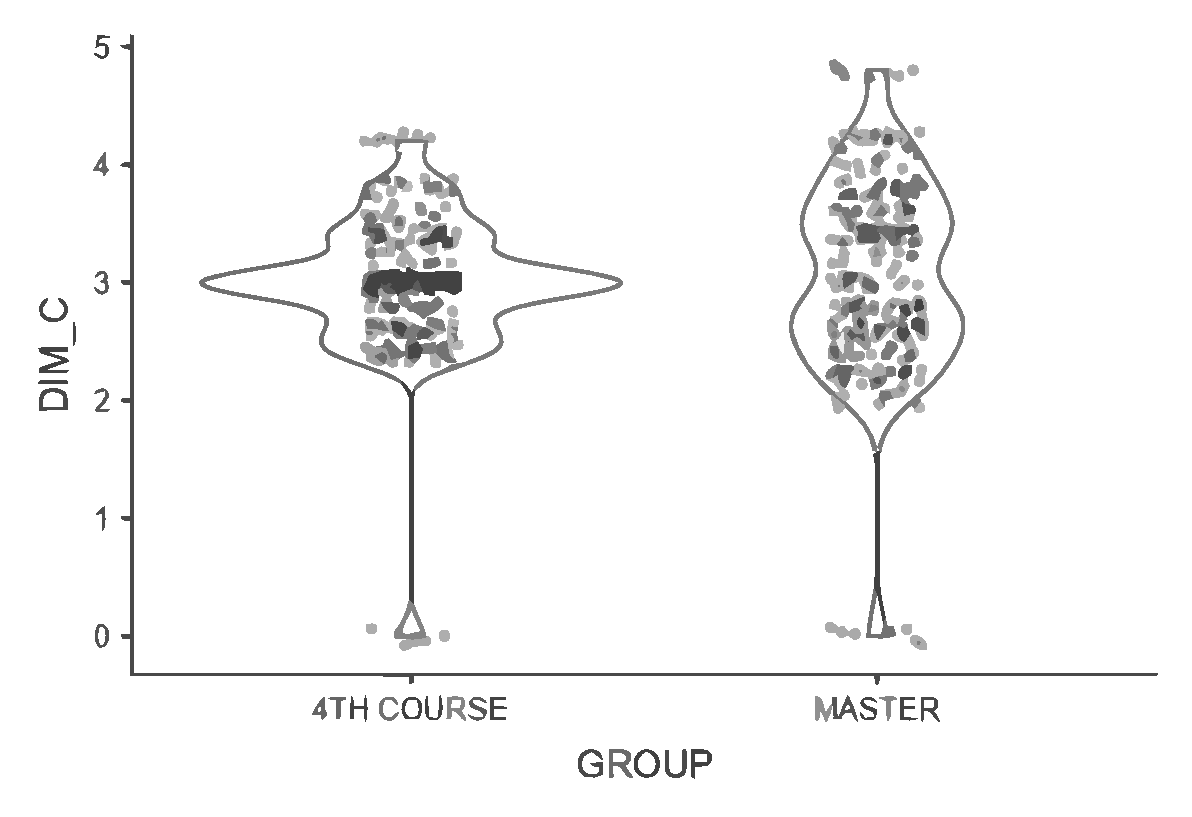
\includegraphics[width=\textwidth]{fig3.jpg}
 \caption{Locais de acesso antes da pandemia.}
 \label{fig03}
 \source{Gráfico elaborado pelos autores.}
\end{minipage}
\end{figure}

\begin{figure}[h!]
\centering
\begin{minipage}{.65\textwidth}
 \includegraphics[width=\textwidth]{fig04.jpg}
 \caption{Otimização do tempo.}
 \label{fig04}
 \source{Gráfico elaborado pelos autores.}
\end{minipage}
\end{figure}

Entre as justificativas apresentadas sobre a preferência pelo uso de dispositivos móveis nas tarefas das disciplinas, os alunos alegaram que esses dispositivos podem ser utilizados em qualquer lugar e em situações que permitem o aproveitamento do tempo para os estudos, conforme excertos \ref{ex12}, \ref{ex13}, \ref{ex14} e \ref{ex15} abaixo. Além disso,  ocupam pouco espaço e contam com bateria de maior duração, permitindo o acesso a multiplataformas da mesma forma que os dispositivos fixos (excerto 16):

\begin{enumerate}[resume]
    \item\label{ex12} Part.\#53: Posso acessar qualquer conteúdo instantaneamente.

    \item\label{ex13} Part.\#66: Algumas vezes não tenho como estudar do meu PC e o smartphone quebra um bom galho, de qualquer lugar, quase qualquer hora.

    \item\label{ex14} Part.\#60: Posso realizar as atividades em qualquer lugar.

    \item\label{ex15} Part.\#40: Posso estudar no ônibus, sendo que fico 2h por dia no transporte, é de grande ajuda.

    \item Part.\#20: Tablets e smartphones ocupam pouco espaço, assim como o Kindle, não necessitam necessariamente de tomadas e permitem o uso de multiplataforma, assim como os computadores de mesa e notebooks, mesmo sendo portáteis.
\end{enumerate}

Como afirma \textcite{gibson1977theory}, o ambiente é repleto de oportunidades de percepção e ação no que diz respeito à interação do indivíduo e ao objeto. Nesse sentido, a presença dos dispositivos móveis no bolso ou na mochila dos universitários pode ser um fator determinante para que se apropriem desses dispositivos para desenvolver atividades de leitura. Ademais, essa apropriação poderá facilitar o acesso às funcionalidades desses dispositivos e possíveis interações com aplicativos que podem auxiliar no desenvolvimento das tarefas. Interações com esses aplicativos são mencionadas pelos estudantes ao serem indagados sobre quais recursos do seu dispositivo móvel (\emph{smartphone} e \emph{tablet}) eles utilizaram para realizar as atividades das disciplinas de Inglês Instrumental. A \Cref{tab01} apresenta os recursos mais utilizados pelos estudantes durante as tarefas das disciplinas de Inglês Instrumental:


\begin{table}[h!]
\centering
\begin{threeparttable}
\caption{Recursos relevantes dos dispositivos móveis.}
\label{tab01}
\begin{tabular}{ll}
\toprule
Recursos mais relevantes dos dispositivos móveis & Quantidade \\
\midrule
Ferramenta de busca & 126 \\
Dicionário on-line ou instalado no aparelho & 70 \\
Google 	tradutor & 97 \\
Caneta 	touch screen & 8 \\
\multicolumn{1}{p{8cm}}{Conversor de texto para voz/voz para texto (para alunos com necessidades especiais)} & 2 \\
\bottomrule
\end{tabular}
\source{Tabela elaborada pelos autores.}
\end{threeparttable}
\end{table}

Limitações quanto ao uso de dispositivos móveis foram investigadas em uma  pergunta do questionário. Questões referentes à limitação quanto ao campo de visão e a possíveis distrações ao realizarem tarefas usando celular foram recorrentes nas respostas dos estudantes. Os excertos a seguir demonstram esses obstáculos:

\begin{enumerate}[resume]
\item Part.\#22: Não, pois eu acabo perdendo mais tempo que ganhando ao me distrair. 
\item Part.\#19: Tela pequena demais para leitura, maior distração por notificações de outros apps.
\end{enumerate}

No que diz respeito às \emph{affordances} que emergem das interações entre os estudantes e os dispositivos móveis durante as atividades da disciplina de leitura, apresentamos um levantamento das características e funcionalidades dos dispositivos, relacionando-as com as \emph{affordances} identificadas a partir da análise das respostas ao questionário aplicado no estudo. Incluímos neste levantamento os trechos dessas respostas indicativos dessas \emph{affordances}:


\begin{table}[h!]
\small
\centering
\begin{threeparttable}
\caption{Affordances relativas às características dos dispositivos móveis.}
\label{tab02}
\begin{tabular}{lp{3cm}p{7.5cm}}
\toprule
\multicolumn{1}{p{3cm}}{Características dos dispositivos} & \emph{Affordances} dos dispositivos móveis para tarefas de leitura & Excertos dos dados gerados pelo questionário \\
\midrule
Mobilidade & Otimizar o tempo de estudo. & 
Part.\#20: “Eu posso estudar em um horário mais confortável e que eu tenha mais disponibilidade”. \newline 
Part.\#24: “Tenho  mobilidade de fazer as tarefas em qualquer lugar”.\newline  
Part.\#31:“O acesso à informação fora de casa facilita o aprendizado”.\newline
Part.\#185: “Tenho uma rotina de vida que não me permite abrir mão de qualquer tempo a mais para estudar. Os dispositivos móveis permitem um melhor aproveitamento do tempo devido ao acesso mais fácil”.\newline
Part.\#76: “Posso estudar no ônibus a caminho do estágio”. \\

Ubiquidade & Consultar o significado das palavras durante a leitura. \newline
Agilizar a resolução de problemas evitando longa espera para sua solução. & 
Part.\#29: “A busca via internet é instantânea e eficaz, reduzindo o tempo de procurar das respostas necessárias”.\newline
Part.\#24: “Com os smartphones tenho recursos que auxiliam no entendimento de forma rápida possibilitando as buscas por palavras ou pelo 	tema rapidamente sem que eu me perca do assunto do texto”. \newline  
Part.\#15: “Acredito que o uso de dispositivos móveis é um facilitador, pois com eles eu possuo uma gama enorme de recursos, o que praticamente anula a possibilidade de uma dúvida persistir por um longo período de tempo”. \newline 
Part.\#03: “Creio que os dispositivos móveis nos fornecem um conhecimento maior daquilo que queremos aprender. Assim sendo, colocando a questão da leitura em Língua Inglesa em pauta, pode-se atestar que o uso de tais ferramentas oferece, ao estudante, uma maior aquisição de explicações e conhecimentos instantâneos sobre o que está sendo abordado no momento do estudo. Concluindo: na minha visão, essa relação gerada é positiva, uma vez que o estudante saiba usar os dispositivos móveis ao seu favor”.  \\
\bottomrule
\end{tabular}
\source{Tabela elaborada pelos autores.}
\end{threeparttable}
\end{table}

Como pode ser observado na \Cref{tab02}, a natureza móvel e ubíqua dos dispositivos móveis tendem a favorecer a emergência de \emph{affordances}. O reconhecimento e percepção dessas características levaram os estudantes a se apropriar desses dispositivos para propósitos que vão além de seu propósito original, como é o caso da otimização do tempo de estudos advinda da possibilidade de desenvolver tarefas a qualquer momento e de qualquer lugar. A ubiquidade desses dispositivos, ou seja, as tecnologias da informação e comunicação móveis, sensores e mecanismos de localização também foram percebidas pelos participantes deste estudo, que se valem da interação desses mecanismos para fazer consultas se significado de palavras acessando o navegador dos seus celulares, traduzir  palavras desconhecidas nos textos em inglês e sanar dúvidas pontuais instantaneamente. A interação com as funcionalidades dos aplicativos também permitiram a emergência de \emph{affordances} como demonstrado na \Cref{tab03}.


\begin{table}[h]
\small
\centering
\begin{threeparttable}
\caption{\emph{Affordances} relativas aos aplicativos.}
\label{tab03}
\begin{tabular}{p{3cm}p{4cm}p{6.6cm}}
\toprule
Funcionalidades / aplicativos dos dispositivos móveis & Affordances dos dispositivos móveis para tarefas de leitura & Excertos dos dados gerados pelos questionários \\
\midrule
Ferramenta de busca & Buscar significados de palavras de forma pontual & Part.\#54: “Quando estou jogando ou lendo um livro em inglês, é extremamente mais cômodo usar o celular para consultar uma tradução ou significado”. \\
Google tradutor \newline Configuração & Solucionar dúvidas por meio de tradução de termos. \newline Adequar o celular ao inglês com vistas ao desenvolvimento de vocabulário. & Part.\#89: “Muitas vezes fico com dúvida sobre alguma palavra e como é fácil pesquisar no tradutor online por dispositivos móveis, faço isso na hora e a palavra e sua tradução acabam se fixando mais na minha mente”. \newline 
Part.\#102: “O google tradutor oferece muito suporte por ser rápido e acessível na tradução de palavras específicas (Google tradutor)”.\newline 
Part.\#38: “Configurei meu celular para língua inglesa há algum tempo	então acabo aprendendo muitas coisas durante pesquisas”. \newline
Part.\#84: “Por muito tempo usei o celular todo em inglês pra forçar que \newline	eu usasse a língua em diversos contextos, pois costumo ter aplicativos diversos”.  \\
Outros aplicativos & Buscar novas oportunidades de aprendizagem & Part.\#73: “Pelo fato de aparelhos móveis serem mais fáceis de se ter por perto em diversos ambientes. Para além dos textos, é um local em que se pode realizar leituras de letras músicas estrangeiras, o que me auxilia no desenvolvimentos das habilidades de leitura; uso de aplicativos, que possuam intuito de manter o contato com a língua estrangeira, como alguns jogos educativos, etc”. \\
\bottomrule
\end{tabular}%
\source{Tabela elaborada pelos autores.}
\end{threeparttable}
\end{table}

A mobilidade e a ubiquidade são características que diferenciam os dispositivos móveis dos fixos e estão diretamente relacionadas ao uso de  funcionalidades/ aplicativos considerando que o uso desses aplicativos está muitas vezes atrelado aos mecanismos das tecnologias da informação e comunicação e à convergência de mídias em eventos que reúnem interações simultâneas entre todos esses aplicativos. Dessa forma, as \emph{affordances} de ‘buscar significados de palavras’ e de ‘solucionar dúvidas por meio de tradução de termos’ emergem das interações com a ferramenta de busca e o Google tradutor que estão interligadas a uma rede de conexões que é acionada durante essas interações. Essas questões igualmente se alinham com as discussões de \textcite[p. 20]{pegrum_mobile_2014}Pegrum, que afirma que a essência da aprendizagem mediada por dispositivos móveis “envolve quando (agora!), quem, o quê e por que, combinados com brevidade, em certo equilíbrio de nem muita e nem tão pouca informação.” Como demonstram as afirmações dos estudantes no questionário, esses dispositivos são utilizados por uma demanda do momento, demanda essa, muitas vezes, de informações pontuais com vistas a soluções imediatas para dificuldades que emergem durante o desenvolvimento das tarefas.

\section{Conclusão}

Neste estudo, discutimos as \emph{affordances} que levam estudantes de graduação a escolherem dispositivos e aplicativos, principalmente móveis, durante o desenvolvimento de tarefas em um curso voltado para o desenvolvimento de estratégias de leitura no contexto de língua inglesa. Os resultados indicam que esses estudantes reconhecem as potencialidades desses recursos e se apropriam deles durante o desenvolvimento das tarefas. Entre as limitações mais relatadas estão dificuldades relativas ao tamanho da tela, desconforto e ergonomia de forma geral, além de falta de otimização do AVA \emph{Moodle} para dispositivos e sistemas móveis. Com relação às \emph{affordances} encontradas neste estudo, podemos citar o uso de apps e sites para buscar significados, principalmente em pesquisas rápidas; respostas para dúvidas a qualquer hora e no próprio ritmo (otimização do tempo de estudo); verificação e aplicação de vocabulários novos, descobrindo seus diferentes significados em contextos distintos. As possibilidades e limitações identificadas durante a apropriação dos dispositivos móveis podem contribuir para futuras investigações voltadas para práticas pedagógicas em contexto digital.

\printbibliography\label{sec-bib}
% if the text is not in Portuguese, it might be necessary to use the code below instead to print the correct ABNT abbreviations [s.n.], [s.l.]
%\begin{portuguese}
%\printbibliography[title={Bibliography}]
%\end{portuguese}


%full list: conceptualization,datacuration,formalanalysis,funding,investigation,methodology,projadm,resources,software,supervision,validation,visualization,writing,review
\begin{contributors}[sec-contributors]
\authorcontribution{Eduardo Simão dos Santos}[datacuration,formalanalysis,investigation,projadm,visualization,writing,review]
\authorcontribution{Júnia de Carvalho Fidelis Braga}[conceptualization,methodology,supervision,review]
\end{contributors}



\end{document}

